\section{Aritmética de la computadora}

Dado que en una computadora todos los números son representados mediante una cantidad de dígitos finita y fija, valores como $\pi$ o $\sqrt{2}$ no se pueden manipular con completa exactitud, pues al ser irracionales tienen infinitos decimales no periódicos. Los irracionales no son los únicos números no representables correctamente en una computadora: aquellos racionales con una cola decimal no periódica suficientemente grande tampoco lo serán. En una computadora sólo se pueden representar con precisión un subconjunto de los números racionales. Esto hace que al hacer cómputos con números reales se genere un error numérico.

\subsection{Representación estándar IEEE}

El estándar fijado por la IEEE contempla varias representaciones que se distinguen por su precisión. Las dos más frecuentemente utilizadas son \emph{single} (32 bits) y \emph{double} (64 bits). Las dos restantes son \emph{half} (16 bits) y \emph{quadruple} (128 bits). Todas estas representaciones son binarias y de punto flotante.

La precisión double tiene la siguiente estructura:

\begin{center}
	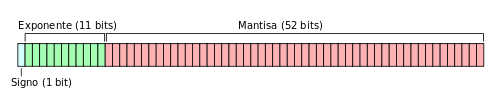
\includegraphics[scale = 0.68]{imagenes/ieee.png}~\\[0.25cm]
\end{center}

\begin{itemize}
	\item \textbf{Signo} ($s$) - 1 bit. El número representado es positivo si $s = 0$ y negativo si no.
	
	\item \textbf{Exponente} ($e$) - 11 bits. La base del exponente es 2. Para poder representar números con valor absoluto menor a 1 es necesario admitir exponentes negativos. Por esto, el exponente está representado en exceso a $2^{10} - 1$, es decir, el exponente del número representado será $(e)_{2} - (2^{10} - 1)$. Como $e$ tiene 11 bits entonces $0 \leq (e)_{2} \leq 2^{11} - 1 \Rightarrow -(2^{10} - 1) \leq (e)_{2} - (2^{10} - 1) \leq 2^{11} - 1 - (2^{10} - 1) \Rightarrow -2^{10} + 1 \leq (e)_{2} - (2^{10} - 1) \leq 2^{10}$.
	
	\item \textbf{Mantisa} ($m$) - 52 bits. Se considera una mantisa normalizada, i. e., el número representado tiene mantisa $(1, m)_{2}$.
\end{itemize}

En definitiva, el número representado es 

\[(-1)^s \cdot (1, m)_2 \cdot 2^{(e)_2 - (2^{10} - 1)}\]

%El mínimo número positivo está dado por $s = 0$, $e = \underbrace{0 \cdots 0}_{11\text{ bits}}$, $m = \underbrace{0 \cdots 0}_{52 \text{ bits}}$, que representa
%
%\[min^{+} = (-1)^0 \cdot 1 \cdot 2^{-1023} = 2^{-1023}\]
%
%El máximo positivo está dado por $s = 0$, $e = \underbrace{1 \cdots 1}_{11\text{ bits}}$, $m = \underbrace{1 \cdots 1}_{52 \text{ bits}}$, que representa
%
%\begin{align*}
%max^{+} &= (-1)^0 \cdot (1, 1 \cdots 1)_{2} \cdot 2^{(1 \cdots 1)_{2} - (2^{10} - 1)}\\
%&= \left(\sum_{i = 0}^{52} \left(\frac{1}{2}\right)^i\right) 2^{2^{11} - 1 - (2^{10} - 1)}\\
%&= \frac{1 - (1 / 2)^{53}}{1 - 1 / 2} 2^{1024}\\
%&= 2^{1024}\left(2 - (1 / 2)^{52}\right)\\
%&\approx 2^{1025}
%\end{align*}
%
%En el estándar IEEE, estos no son en realidad el mínimo y máximo valor positivo representable, debido a que los exponentes $e = 0$ y $e = \underbrace{1 \cdots 1}_{11 \text{ bits}}$ están reservados para valores especiales. De todos modos, $min^+$ y $max^+$ se aproximan bastante a los reales, y sirven para hacernos una idea de cuán chico o cuán grande puede ser un número representable en este sistema.
%
%Dado que el bit $s$ determina el signo del número, la representación es simétrica respecto del cero. Por lo tanto, los números negativos representables de menor y mayor absoluto son aproximadamente $- min^+$ y $- max^+$ respectivamente.

\begin{defi}
Decimos que un cómputo genera \emph{underflow} si su resultado es menor que el mínimo positivo representable, en módulo. Análogamente, decimos que genera \emph{overflow} si su resultado es mayor que el máximo positivo representable, en módulo.
\end{defi}

\subsection{Aproximación de los reales mediante números de máquina}

En esta sección estudiaremos cuán eficaz es la aproximación de un número real mediante un sistema con las características del presentado previamente. El tipo de sistemas a los que nos referimos son representaciones de punto flotante con una longitud de mantisa fija y exponente acotado.

Supongamos que nuestro conjunto de números de máquina es

\[\mathcal{M} = \{x \in \mathbb{R} : x = \pm (0, d_1 d_2 \cdots d_k) \cdot 10^e, 0 \leq d_i \leq 9, d_1 \neq 0, e_1 \leq e \leq e_2\}\]

dadas ciertas constantes $k$, $e_1$ y $e_2$. Esta es una representación normalizada con mantisa de $k$ dígitos y exponente entre $e_1$ y $e_2$. Es un sistema decimal y no binario como el de la IEEE, porque así será más fácil razonar sobre él. Todos los resultados que veremos en esta sección aplican, mutatis mutandi, a un sistema similar que utilice una base $b > 1$ cualquiera.

También por simplicidad, asumiremos que $e_1 = -\infty$ y $e_2 = +\infty$. Esto ahorra hablar del rango en el que corre el exponente, lo cual, como veremos, no hace a la esencia de los resultados.

\begin{defi}
Si $x \in \mathbb{R}$ es cualquiera, no necesariamente de máquina, llamamos $fl(x)$ a la aproximación de $x$ vía números de máquina. 
\end{defi}

Es definición depende del modo en que realicemos la aproximación. Consideremos la escritura

\[x = (0, d_1 \cdots d_kd_{k + 1} \cdots) \cdot 10^e\]
	
con $d_1 \neq 0$ (esta escritura es única dado que $d_1 \neq 0$). Entonces dos formas de aproximar $x$ son:

\begin{itemize}
	\item \textbf{Truncamiento.} Simplemente descartamos los dígitos $d_{k + 1}, d_{k + 2}, \cdots$, para obtener
	
	\[fl(x) = (0, d_1 \cdots d_k) \cdot 10^e\]

	\item \textbf{Redondeo.} Si $d_{k + 1} < 5$ entonces truncamos. Si no, sumamos $0,\underbrace{0 \cdots 05}_{k + 1 \text{ dígitos}} \cdot 10^e = 5 \cdot 10^{-(k + 1)} \cdot 10^e$ a $x$ y truncamos. En este último caso lo que queda es
	
	\[fl(x) = [(0, d_1 \cdots d_k) + 10^{-k}] \cdot 10^e\]

\end{itemize}

Una forma equivalente de enunciar estos criterios es la siguiente. Sea $x^{-}$ es el máximo número de máquina menor o igual que $x$. Análogamente, sea $x^{+}$ el mínimo número de máquina mayor o igual que $x$. Entonces, el truncamiento aproxima por $x^-$ mientras que el redondeo aproxima por aquel valor de $x^-$ o $x^+$ más cercano a $x$.

En general, las computadoras utilizan la aproximación por redondeo.

\subsection{Distribución de los números de máquina sobre la recta real}

\begin{obs}
Un número de máquina con exponente $e$ cae en el intervalo $[10^{e - 1}, 10^e)$.
\end{obs}

\begin{lema}
\label{lema:suc}
Dado $x \in \mathcal{M}$ con exponente $e$, el número de máquina que lo sucede es $x' = x + 10^{-k} \cdot 10^e$.

\begin{proof}
Por la observación anterior, $x$ cae en el intervalo $[10^{e - 1}, 10^e)$. Si $x$ es el máximo número de máquina en dicho intervalo, entonces $x'$ es el número de máquina más pequeño en $[10^e, 10^{e + 1})$, i. e., $x' = (0,1) \cdot 10^{e + 1}$. En caso contrario, el sucesor $x'$ también cae en $[10^{e - 1}, 10^e)$, con lo cual tiene exponente $e$. Lo mínimo que puede incrementarse la mantisa de $x$ es $0,\underbrace{0 \cdots 01}_{k \text{ dígitos}}$, con lo cual $x' = x + (0,\underbrace{0 \cdots 01}_{k \text{ dígitos}}) \cdot 10^e = x + 10^{-k} \cdot 10^e$.
\end{proof}
\end{lema}

La distribución de $\mathcal{M}$ no es uniforme sobre la recta real. Para ver por qué, contemos la cantidad de números de máquina que hay en el intervalo $[10^{i}, 10^{i + 1})$ con $i \in \mathbb{Z}$ una constante entera.

\begin{propo}
\label{propo:dist}
La cantidad de números de máquina $x \in \mathcal{M}$ tal que $x \in [10^i, 10^{i + 1})$ es $9 \cdot 10^{k - 1}$.

\begin{proof}
El menor número de máquina en $[10^{i}, 10^{i + 1})$ es $(0,1) \cdot 10^{i + 1} = 10^{i}$, y el mayor es $(0,99\cdots 99) \cdot 10^{i + 1}$. Entre estos dos están

\begin{center}
$(0,10\cdots 00) \cdot 10^{i + 1}$\\
$(0,10\cdots 01) \cdot 10^{i + 1}$\\
	$\vdots$\\
$(0,99\cdots 98) \cdot 10^{i + 1}$\\
$(0,99\cdots 99) \cdot 10^{i + 1}$\\
\end{center}

Observemos que estos son todos los números de máquina positivos con exponente $i + 1$. Afirmamos que no hay otros números de máquina en $[10^i, 10^{i + 1})$. Si un número en $\mathcal{M}$ positivo tiene exponente menor o igual que $i$, como la mantisa es estrictamente menor que 1, entonces el número será estrictamente menor que $10^i$. En caso contrario, si tiene exponente mayor o igual que $i + 2$, como el primer dígito decimal de la mantisa es no nulo, el número será al menos $10^{i + 1}$.

Para ver cuántos números hay en esta lista, notemos que hay tantos como números enteros entre $10^{k - 1}$ y $10^{k} - 1$, y estos son $9 \cdot 10^{k - 1}$.
\end{proof}
\end{propo}

\begin{coro}
Los números de máquina no están uniformemente distribuidos.

\begin{proof}
Como $\#(\mathcal{M} \cap [10^i, 10^{i + 1})) = 9 \cdot 10^{k - 1}$ no depende de $i$, resulta que en los intervalos $[1, 10)$, $[10, 100)$, $[100, 1000)$, $\cdots$, $[10^i, 10^{i + 1})$, $\cdots$, hay igual cantidad de números de máquina.
\end{proof}
\end{coro}

Intuitivamente, cuanto más nos alejemos de 0, más esparcidos estarán los números de máquina. Lo próximo que queremos es medir cuán esparcidos están, según el intervalo $[10^i, 10^{i + 1})$ en el que caigan.

\begin{lema}
Sea $x \in \mathcal{M} \cap [10^i, 10^{i + 1})$ y sea $x'$ su sucesor. Entonces $x' - x = 10^{i + 1 - k}$.

\begin{proof}
Como el exponente de $x$ es $i + 1$ entonces $x' = x + 10^{-k} \cdot 10^{i + 1}$, y concluimos $x' - x = 10^{i + 1 - k}$.
\end{proof}
\end{lema}

\begin{coro}
En cada intervalo $[10^i, 10^{i + 1})$ los números de máquina consecutivos estan equiespaciados.
\end{coro}

Más aún, a medida que $i$ crece, la brecha entre elementos consecutivos en $[10^i, 10^{i + 1})$ se hace mayor. De aquí se deduce que la distribución de los números de máquina tiene el siguiente aspecto
\\[0.5cm]
\begin{figure}[h]
\centering
\input{imagenes/distribucion.pdf_tex}
\end{figure}\\[0.5cm]

Esta distribución puede parecer extraña. Contrariamente a lo intuitivo, que haría pensar que una distribución uniforme sería más útil, esta distribución exponencial de los números de máquina resulta práctica pues se basa en la idea de que cuanto más chicos sean los números del rango en el que estamos trabajando, más pequeñas serán las variaciones que estaremos interesados en hacer. Contrariamente, cuanto más grandes sean los números con los que trabajemos, más grandes serán las variaciones con las que vayamos a trabajar. Esta noción se formaliza en la siguiente sección.

\subsection{Error absoluto y error relativo}

\begin{defi} Sea $x \in \mathbb{R}$. Sea $x^* \in \mathbb{R}$ un valor que pretende aproximar a $x$. 
\begin{itemize}
	\item El error absoluto de aproximar $x$ por $x^*$ es $|x - x^*|$.
	\item El error relativo de aproximar $x$ por $x^*$ es $\frac{|x - x^*|}{|x|}$.
\end{itemize}
\end{defi}

Notemos que la diferencia entre estas dos medidas de error, es que el absoluto no contempla el tamaño del valor que estamos aproximando mientras que el relativo sí lo hace. Esto determina que, en general, el error absoluto no sea una buena medida para el error, puesto que en ciertos contextos podemos tener un error absoluto aparentemente grande aunque la aproximación sea buena (por ejemplo, si aproximáramos la distancia entre la Tierra y la Luna con un error absoluto de 1000m) y en otros contextos podemos tener un error absoluto aparentemente chico aunque la aproximación sea mala (por ejemplo, si aproximáramos el perímetro de una célula vegetal con un error absoluto de 1mm).

Supongamos que queremos aproximar una magnitud que vale $x = 1000$, y nos piden que el error relativo sea a lo sumo $0,01$. Si nuestra medición es $x^* = 990$ entonces el error relativo será

\[\frac{|x - x^*|}{|x|} = \frac{10}{1000} = 0,01\]

con lo cual esta medición satisface lo pedido. Es fácil ver que cualquiera sea $x^* \in [990, 1010]$ cumple.

Supongamos que ahora estamos buscando medir una magnitud $x = 10$. La precisión buscada es la misma que antes, lo cual tiene sentido pues está expresada en términos relativos. Notemos que la medición $x^* = 9$ no será aceptada, porque el error relativo será de $0.1$. Refinando la medición a $x^* = 9.9$ conseguimos un error relativo de $0.01$ y es claro que cualquier valor $x^* \in [9.9; 10.1]$ no sobrepasa este error.

En ambas situaciones los errores relativos eran los mismos, sin embargo la diferencia en valor absoluto entre $x$ y los valores de $x^*$ aceptados era mucho mayor en el primer caso que en el segundo caso. La discusión del final de la sección anterior cobra ahora mucho más sentido.

A continuación estudiamos el error relativo al aproximar un número real por un número de máquina.

\begin{propo}
Si $fl(x)$ se obtiene truncando $x$ entonces

\[\frac{|x - fl(x)|}{|x|} \leq 10^{1 - k}\]

\begin{proof}
Supongamos sin pérdida de generalidad que $x > 0$. Sea $x = (0,d_1 \cdots d_k d_{k + 1} \cdots) \cdot 10^e$. Entonces

\begin{align*}
\frac{|x - fl(x)|}{|x|} &= \frac{|(0,d_1\cdots d_k d_{k + 1}\cdots) \cdot 10^e - (0,d_1 \cdots d_k) \cdot 10^e|}{|(0,d_1\cdots d_k d_{k + 1} \cdots) \cdot 10^e|}\\
&= \frac{(0,0\cdots 0 d_{k + 1} d_{k + 2} \cdots )}{(0,d_1 \cdots d_k d_{k + 1} \cdots)}
\end{align*}

Como $(0,d_1 \cdots d_k d_{k + 1} \cdots) \geq 0,1 = 10^{-1}$ y $(0,0\cdots 0 d_{k + 1}d_{k + 2}\cdots) \leq 0,\underbrace{0\cdots 01}_{k \text{ dígitos}} = 10^{-k}$, entonces

\[\frac{|x - fl(x)|}{|x|} \leq 10 \cdot 10^{-k} = 10^{1 - k}\]

\end{proof}
\end{propo}

\begin{propo}
\label{propo:er}
Si $fl(x)$ se obtiene redondeando $x$ entonces

\[\frac{|x - fl(x)|}{|x|} \leq \frac{1}{2} \cdot 10^{1 - k}\]

\begin{proof}
Separamos en casos, según el valor de $d_{k + 1}$.

Si $d_{k + 1} < 5$ entonces $fl(x) = (0,d_1 \cdots d_k) \cdot 10^e$. Entonces, haciendo la misma cuenta que antes,

\[\frac{|x - fl(x)|}{|x|} = \frac{(0,0\cdots 0 d_{k + 1} d_{k + 2} \cdots )}{(0,d_1 \cdots d_k d_{k + 1} \cdots)}\]

Como $d_{k + 1} < 5$ entonces $(0,0\cdots 0 d_{k + 1} d_{k + 2} \cdots) \leq 5 \cdot 10^{-(k + 1)}$. Luego

\[\frac{|x - fl(x)|}{|x|} \leq 5 \cdot 10^{-(k + 1)} \cdot 10 = \frac{10}{2} \cdot 10^{-k} = \frac{1}{2} \cdot 10^{1 - k}\]

Veamos el caso $d_{k + 1} \geq 5$. Ahora tenemos $fl(x) = [(0, d_1 \cdots d_k) + 10^{-k}] \cdot 10^e$. Entonces

\begin{align*}
\frac{|x - fl(x)|}{|x|} &= \frac{|(0,d_1\cdots d_k d_{k + 1}\cdots) - [(0,d_1\cdots d_k) + 10^{-k}]|}{(0,d_1\cdots d_k d_{k + 1} \cdots)}\\
&= \frac{|(0,0\cdots 0d_{k + 1}d_{k + 2}\cdots) - 10^{-k}|}{(0,d_1\cdots d_k d_{k + 1} \cdots)}\\
&= \frac{10^{-k} - (0,0\cdots 0d_{k + 1}d_{k + 2}\cdots)}{(0,d_1\cdots d_k d_{k + 1} \cdots)}\\
&= \frac{(0,0\cdots 0(9 - d_{k + 1})(9 - d_{k + 2}) \cdots)}{(0,d_1\cdots d_k d_{k + 1} \cdots)}
\end{align*}

Como $d_{k + 1} \geq 5$ entonces $(0,0\cdots 0(9 - d_{k + 1})(9 - d_{k + 2}) \cdots ) \leq (0,\underbrace{0\cdots 0}_{k \text{ dígitos}}499\cdots) = 5 \cdot 10^{-(k + 1)}$. Luego

\[\frac{|x - fl(x)|}{|x|} \leq 5 \cdot 10^{-(k + 1)} \cdot 10 = \frac{1}{2} \cdot 10^{1 - k}\]

\end{proof}
\end{propo}

\begin{coro}
En una máquina con representación de punto flotante decimal con mantisa de $k$ dígitos, el error de redondeo es $\mathcal{O}(10^{-k})$.
\end{coro}

El máximo error relativo que se puede cometer, según lo calculado en la Proposición \ref{propo:er}, tiene un nombre particular.

\subsection{Epsilon de máquina}

\begin{defi}
Llamamos epsilon de máquina al máximo error relativo que puede cometerse por redondeo. Lo notamos $\varepsilon$.
\end{defi}

En el caso de la máquina $\mathcal{M}$ con la que venimos trabajando, el epsilon de máquina es $\varepsilon = \frac{1}{2} \cdot 10^{1 - k}$.

\begin{propo}
$\varepsilon$ es el mínimo real positivo $x$ tal que $fl(1 + x) \neq 1$.

\begin{proof}
La observación clave es que el número representable que sigue al 1 es $1 + 10^{-k} \cdot 10 = 1 + 10^{1 - k}$ (Lema \ref{lema:suc}). Entonces, el punto medio entre 1 y su sucesor es $1 + \frac{1}{2} \cdot 10^{1 - k}$. De aquí se deduce que si $0 \leq x < \frac{1}{2} \cdot 10^{1 - k}$ entonces al redondear $1 + x$ obtenemos $fl(1 + x) = 1$, y si $x = \frac{1}{2} \cdot 10^{1 - k}$ y redondeamos $1 + x$ obtenemos el sucesor. Entonces $x = \frac{1}{2} \cdot 10^{1 - k} = \varepsilon$ es el mínimo que cumple lo buscado.
\end{proof}
\end{propo}

\begin{obs}
La validez de este resultado proviene de la fuerte relación que hay entre la cota superior para el error relativo y la distancia entre 1 y el número de máquina que lo sucede.
\end{obs}

\begin{obs}
El epsilon de máquina no tiene ninguna relación con el mínimo real positivo representable. De hecho, el mínimo representable depende del rango en el que se mueve el exponente, y no de la precisión de la mantisa.
\end{obs}

%\begin{propo}
%Sea $\alpha \in \mathcal{M}$ cualquiera, que tiene exponente $e$. El mínimo real positivo $x$ tal que $fl(\alpha + x) \neq \alpha$ es $x = \varepsilon \cdot 10^{e - 1} = \mathcal{O}(\varepsilon |\alpha|)$.

%\begin{proof}
%El sucesor de $\alpha$ es $\alpha + 10^{-k} \cdot 10^e$. El punto medio entre estos dos números de máquina será $\alpha + \frac{1}{2} \cdot 10^{-k} \cdot 10^e = \alpha + \varepsilon \cdot 10^{e - 1}$. Entonces el mínimo $x$ será dicho punto medio $x = \varepsilon \cdot 10^{e - 1}$. 
%\end{proof}
%\end{propo}

La noción de $\varepsilon$ permite dar cotas superiores sobre el error cometido al realizar distintas operaciones en una máquina, independientemente de las características del sistema de representación de números que utilice la misma. Las cuatro operaciones estándar que realiza una computadora son,

\[x \oplus y = fl(fl(x) + fl(y))\]
\[x \ominus y = fl(fl(x) - fl(y))\]
\[x \otimes y = fl(fl(x) \times fl(y))\]
\[x \oslash y = fl(fl(x) / fl(y))\]

que representan, respectivamente, la suma, la resta, el producto y el cociente de dos números reales $x$ e $y$.

\begin{propo}
Sean $x, y \in \mathbb{R}$ no nulos, con igual signo. En cualquier máquina con suma $\oplus$, que utilice redondeo, vale

\[\frac{|(x + y) - (x \oplus y)|}{|x + y|} \leq 2\varepsilon + \varepsilon^2\]

\begin{proof}
En efecto,

\begin{align*}
\frac{|(x + y) - (x \oplus y)|}{|x + y|} &= \frac{|(x + y) - (x \oplus y)|}{|x + y|}\\
&= \frac{|(x + y) - fl(fl(x) + fl(y))|}{|x + y|}\\
&= \frac{|x + y - (fl(x) + fl(y)) + (fl(x) + fl(y)) - fl(fl(x) + fl(y))|}{|x + y|}\\
&= \frac{\left|x\frac{x - fl(x)}{x} + y \frac{y - fl(y)}{y} + (fl(x) + fl(y)) \frac{fl(x) + fl(y) - fl(fl(x) + fl(y))}{fl(x) + fl(y)}\right|}{|x + y|}\\
&\leq \frac{1}{|x + y|} \left(|x| \frac{|x - fl(x)|}{|x|} + |y| \frac{|y - fl(y)|}{|y|} + |fl(x) + fl(y)| \frac{|fl(x) + fl(y) - fl(fl(x) + fl(y))|}{|fl(x) + fl(y)|}\right)\\
&\leq \frac{1}{|x + y|} \left(|x|\varepsilon + |y| \varepsilon + |fl(x) + fl(y)| \varepsilon \right)\\
&= \frac{1}{|x + y|}\left(|x| + |y| + |fl(x) + fl(y)| \right)\varepsilon\\
&= \frac{1}{|x + y|}\left(|x| + |y| + \left|x \frac{fl(x) - x}{x} + y \frac{fl(y) - y}{y} + x + y\right|\right)\varepsilon\\
&\leq \frac{1}{|x + y|}\left(|x| + |y| + |x|\frac{|x - fl(x)|}{|x|} + |y| \frac{|y - fl(y)|}{|y|} + |x| + |y|\right)\varepsilon\\
&\leq \frac{1}{|x + y|}\left(2|x| + 2|y| + |x|\varepsilon + |y|\varepsilon \right)\varepsilon\\
&=\frac{1}{|x + y|}(|x| + |y|)(2 + \varepsilon)\varepsilon\\
&=\frac{|x| + |y|}{|x + y|}(2\varepsilon + \varepsilon^2)
\end{align*}

Como $x$ e $y$ tienen igual signo, $\frac{|x| + |y|}{|x + y|} = 1$, lo cual termina la demostración.
\end{proof}
\end{propo}

%\begin{propo}
%Sean $x, y \in \mathbb{R}$ no nulos. En cualquier máquina con producto $\otimes$, que utilice redondeo, vale

%\[\frac{|xy - x \otimes y|}{|xy|} \leq 3\varepsilon + 3\varepsilon^2 + \varepsilon^3\]

%\begin{proof}
%En efecto,

%\begin{align*}
%\frac{|xy - x \otimes y|}{|xy|} &= \frac{|xy - fl(fl(x)fl(y))|}{|xy|}\\
%&=\frac{\left|y(x - fl(x)) + fl(x)(y -fl(y)) + (fl(x)fl(y))\frac{fl(x)fl(y) -fl(fl(x)fl(y))}{fl(x)fl(y)}\right|}{|xy|}\\
%&\leq \frac{|x - fl(x)|}{|x|} + \frac{|fl(x)|}{|x|}\frac{|y - fl(y)|}{|y|} + \frac{|fl(x)fl(y)|}{|xy|} \frac{|fl(x)fl(y) - fl(fl(x)fl(y))|}{|fl(x)fl(y)|}\\
%&\leq \varepsilon + \frac{|fl(x)|}{|x|}\varepsilon + \frac{|fl(x)fl(y)|}{|xy|}\varepsilon\\
%&= \left(1 + \frac{|fl(x)|}{|x|} + \frac{|fl(x)|}{|x|}\frac{|fl(y)|}{|y|}\right)\varepsilon
%\end{align*}

%Notemos que $\frac{|fl(x)|}{|x|} = \frac{|fl(x) - x + x|}{|x|} \leq \frac{|fl(x) - x|}{|x|} + 1 \leq \varepsilon + 1$, y análogamente con $y$. Entonces

%\begin{align*}
%\frac{|xy - x \otimes y|}{|xy|} &\leq (1 + (\varepsilon + 1) + (\varepsilon + 1)^2)\varepsilon\\
%&= 3\varepsilon + 3\varepsilon^2 + \varepsilon^3
%\end{align*}

%\end{proof}
%\end{propo}

%Comparemos las cotas obtenidas para las dos operaciones. Como $\varepsilon$ es muy chico, tiene sentido descartar todos los términos salvo los lineales. Concluimos que, a lo sumo, la suma (de números de igual signo) introduce un error aproximado $2\varepsilon$ y el producto un error aproximado $3\varepsilon$.

\subsection{Errores de redondeo clásicos}

\subsubsection{Suma de números de órdenes muy distintos}

Supongamos que tenemos un número real de valor absoluto pequeño, y otro de valor absoluto grande. Entonces la suma de máquina de los dos puede hacer que el más pequeño desaparezca.

Para ejemplificar, supongamos que nuestra aritmética tiene una precisión de $k = 5$ dígitos de mantisa. Sean $x = 0,88888888 \cdot 10^7$ e $y = 0,1 \cdot 10^2$. Entonces

\begin{align*}
x \oplus y &= fl(fl(x) + fl(y))\\
&= fl(0,88888 \cdot 10^7 + 0,1 \cdot 10^2)\\
&= fl(0,888881 \cdot 10^7)\\
&= 0,88888 \cdot 10^7
\end{align*}

El término $x$ ha absorbido a $y$. 

\subsubsection{Resta de números cercanos}

Al restar dos números cercanos, el resultado estará próximo a cero, lo que puede ocasionar que se pierdan dígitos significativos. Este fenómeno se conoce como \emph{cancelación catastrófica}, y tiene un gran impacto en el error relativo.

A modo de ejemplo, supongamos nuevamente que la precisión es de $k = 5$ dígitos, y sean que $x = 0,12346923$ e $y = 0,12345175$ entonces

\begin{align*}
x \ominus y &= fl(fl(x) - fl(y))\\
&= fl(0,12347 - 0,12345)\\
&= fl(0,00002)\\
&= 0,00002
\end{align*}

Sin embargo $x - y = 0,00001748$, lo que muestra que hemos perdido 3 dígitos significativos del resultado en la operación con redondeo.

\subsubsection{Multiplicación por números grandes o dividisión por números pequeños}

En este caso, se produce una amplificación del error absoluto acarreado. Supongamos que $x^*$ es una aproximación de máquina de $x$. Dividiendo a $x^*$ por un número muy pequeño, digamos $10^{-n}$ para cierto $n > 0$, obtenemos el número de máquina $x^* / 10^{-n}$ que aproxima a $x / 10^{-n}$ con un error absoluto de

\[|x^* / 10^{-n} - x / 10^{-n}| = |x^* - x| \cdot 10^{n}\]

El error absoluto $|x^* - x|$ del primer redondeo se ve amplificado en un factor de $10^n$.

\subsection{Generalización}

Como hemos dicho al principio de esta sección, hemos estudiado la representación de los números de máquina utilizando un sistema de base 10 exclusivamente por comodidad. Todos los resultados que vimos son fácilmente generalizables a una base arbitraria $b > 1$. A modo de ejemplo, en un conjunto análogo a $\mathcal{M}$ pero de base 2, el epsilon de máquina resulta ser $\varepsilon = \frac{1}{2} \cdot 2^{1 - k} = 2^{-k}$. 

Otro ejemplo interesante es la representación IEEE de precisión doble, cuyo conjunto de números de máquina es similar a $\mathcal{M}$ pero es de base 2 y tiene $k = 52 + 1$ dígitos de precisión (52 dígitos de mantisa más 1 dígito de precisión que agrega la normalización de la misma). Entonces, el epsilon de máquina en una computadora que use representación IEEE de precisión doble será $\varepsilon = 2^{-53}$. Éste es el máximo error relativo que una computadora típica cometerá por redondeo.